\section{Iteration 6: Decomposition of the Scheduler for Anomaly Detection}
\label{add:it6}

\subsection{Step 1: Identify candidate drivers}
\label{add:it6/drivers}

% TODO

\subsection{Step 2: Choose design concepts}
\label{add:it6/concepts}

% TODO 

\subsection{Step 3: Instantiate architectural elements and allocate responsibilities}
\label{add:it6/elements}

% TODO

\npar An overview of the instantiated child components of the Anomaly Detection
Scheduler is shown in \ref{fig:it6/elements}.

\begin{figure}[H]
	\begin{centering}
		% TODO Figure
		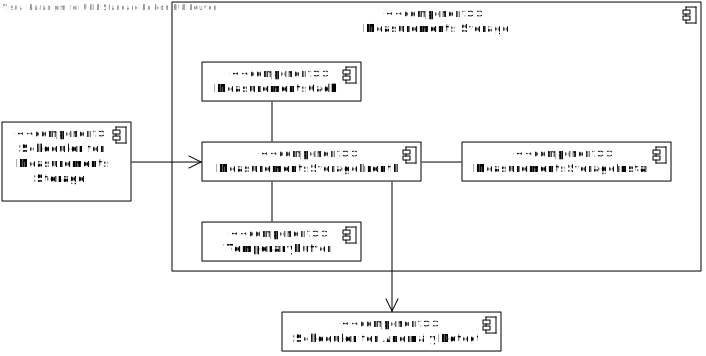
\includegraphics[width=\textwidth]{figs/add-it4-elements.pdf}
		\caption{Overview of all instantiated child elements in the Anomaly
		Detection Unit}
		\label{fig:it6/elements}
	\end{centering}
\end{figure}

\subsection{Step 4: Define interfaces for instantiated elements}
\label{add:it6/interfaces}

% TODO

\begin{figure}[H]
	\begin{centering}
		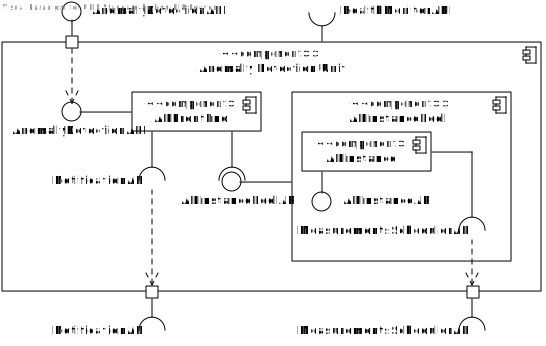
\includegraphics[width=\textwidth]{figs/add-it6-interfaces.pdf}
		\caption{Overview of the interfaces and components in the Anomaly Detection
		Unit}
		\label{fig:it6/interfaces}
	\end{centering}
\end{figure}

\subsection{Step 5: Verify and refine}
\label{add:it6/verification}

% TODO verify & refine
